\documentclass{article}

\usepackage[preprint]{neurips_2026}

\usepackage[utf8]{inputenc}
\usepackage[T1]{fontenc}
\usepackage{hyperref}
\usepackage{url}
\usepackage{booktabs}
\usepackage{amsfonts}
\usepackage{amsmath}
\usepackage{amssymb}
\usepackage{nicefrac}
\usepackage{microtype}
\usepackage{xcolor}
\usepackage{graphicx}

\newcommand{\nRawJan}{1,497,237}
\newcommand{\nGamesJan}{1,478,833}
\newcommand{\nRawFeb}{1,495,553}
\newcommand{\nGamesFeb}{1,476,869}
\newcommand{\nRawMar}{1,742,733}
\newcommand{\nGamesMar}{1,722,169}
\newcommand{\nDaysFeb}{28}
\newcommand{\nPlayersFeb}{40,645}
\newcommand{\nDaysMar}{31}
\newcommand{\nPlayersMar}{46,405}
\newcommand{\nDaysJan}{31}
\newcommand{\llEloFeb}{0.6265}
\newcommand{\llEloMar}{0.6257}
\newcommand{\llFloorFeb}{0.6924}
\newcommand{\llFloorMar}{0.6925}
\newcommand{\llBaseFeb}{0.6220}
\newcommand{\llBaseMar}{0.6213}
\newcommand{\llPooledFeb}{0.6220}
\newcommand{\llPooledMar}{0.6213}
\newcommand{\llRatingFeb}{0.6220}
\newcommand{\llRatingMar}{0.6213}
\newcommand{\llSplineFeb}{0.6218}
\newcommand{\llSplineMar}{0.6211}
\newcommand{\llBoostFeb}{0.6217}
\newcommand{\llBoostMar}{0.6210}
\newcommand{\llOrdinalFeb}{0.6220}
\newcommand{\llOrdinalMar}{0.6213}
\newcommand{\dEloPooledFeb}{$-$44.6}
\newcommand{\dEloPooledFebLo}{$-$48.9}
\newcommand{\dEloPooledFebHi}{$-$40.5}
\newcommand{\dEloPooledFebAbs}{44.6}
\newcommand{\dEloPooledFebPm}{4.2}
\newcommand{\dEloBaseFeb}{$-$45.0}
\newcommand{\dEloBaseFebLo}{$-$49.3}
\newcommand{\dEloBaseFebHi}{$-$40.8}
\newcommand{\dEloBaseFebAbs}{45.0}
\newcommand{\dEloBaseFebPm}{4.3}
\newcommand{\dEloRatingFeb}{$-$45.2}
\newcommand{\dEloRatingFebLo}{$-$49.7}
\newcommand{\dEloRatingFebHi}{$-$40.9}
\newcommand{\dEloRatingFebAbs}{45.2}
\newcommand{\dEloRatingFebPm}{4.4}
\newcommand{\dEloSplineFeb}{$-$46.9}
\newcommand{\dEloSplineFebLo}{$-$51.6}
\newcommand{\dEloSplineFebHi}{$-$42.3}
\newcommand{\dEloSplineFebAbs}{46.9}
\newcommand{\dEloSplineFebPm}{4.6}
\newcommand{\dEloBoostFeb}{$-$48.1}
\newcommand{\dEloBoostFebLo}{$-$53.1}
\newcommand{\dEloBoostFebHi}{$-$43.4}
\newcommand{\dEloBoostFebAbs}{48.1}
\newcommand{\dEloBoostFebPm}{4.8}
\newcommand{\dEloOrdinalFeb}{$-$45.0}
\newcommand{\dEloOrdinalFebLo}{$-$49.2}
\newcommand{\dEloOrdinalFebHi}{$-$40.8}
\newcommand{\dEloOrdinalFebAbs}{45.0}
\newcommand{\dEloOrdinalFebPm}{4.2}
\newcommand{\dEloFloorFeb}{659.5}
\newcommand{\dEloFloorFebLo}{627.6}
\newcommand{\dEloFloorFebHi}{692.8}
\newcommand{\dEloFloorFebAbs}{659.5}
\newcommand{\dEloFloorFebPm}{32.6}
\newcommand{\dBasePooledFeb}{0.3}
\newcommand{\dBasePooledFebLo}{0.1}
\newcommand{\dBasePooledFebHi}{0.6}
\newcommand{\dBasePooledFebAbs}{0.3}
\newcommand{\dBasePooledFebPm}{0.2}
\newcommand{\dBaseBaseFeb}{0.0}
\newcommand{\dBaseBaseFebLo}{0.0}
\newcommand{\dBaseBaseFebHi}{0.0}
\newcommand{\dBaseBaseFebAbs}{0.0}
\newcommand{\dBaseBaseFebPm}{0.0}
\newcommand{\dBaseRatingFeb}{$-$0.3}
\newcommand{\dBaseRatingFebLo}{$-$0.6}
\newcommand{\dBaseRatingFebHi}{0.0}
\newcommand{\dBaseRatingFebAbs}{0.3}
\newcommand{\dBaseRatingFebPm}{0.3}
\newcommand{\dBaseSplineFeb}{$-$1.9}
\newcommand{\dBaseSplineFebLo}{$-$2.8}
\newcommand{\dBaseSplineFebHi}{$-$1.1}
\newcommand{\dBaseSplineFebAbs}{1.9}
\newcommand{\dBaseSplineFebPm}{0.9}
\newcommand{\dBaseBoostFeb}{$-$3.1}
\newcommand{\dBaseBoostFebLo}{$-$4.2}
\newcommand{\dBaseBoostFebHi}{$-$2.1}
\newcommand{\dBaseBoostFebAbs}{3.1}
\newcommand{\dBaseBoostFebPm}{1.1}
\newcommand{\dBaseOrdinalFeb}{0.0}
\newcommand{\dBaseOrdinalFebLo}{0.0}
\newcommand{\dBaseOrdinalFebHi}{0.0}
\newcommand{\dBaseOrdinalFebAbs}{0.0}
\newcommand{\dBaseOrdinalFebPm}{0.0}
\newcommand{\dBaseFloorFeb}{704.5}
\newcommand{\dBaseFloorFebLo}{674.5}
\newcommand{\dBaseFloorFebHi}{736.4}
\newcommand{\dBaseFloorFebAbs}{704.5}
\newcommand{\dBaseFloorFebPm}{31.0}
\newcommand{\dEloPooledMar}{$-$43.4}
\newcommand{\dEloPooledMarLo}{$-$48.0}
\newcommand{\dEloPooledMarHi}{$-$38.9}
\newcommand{\dEloPooledMarAbs}{43.4}
\newcommand{\dEloPooledMarPm}{4.5}
\newcommand{\dEloBaseMar}{$-$43.8}
\newcommand{\dEloBaseMarLo}{$-$48.5}
\newcommand{\dEloBaseMarHi}{$-$39.3}
\newcommand{\dEloBaseMarAbs}{43.8}
\newcommand{\dEloBaseMarPm}{4.6}
\newcommand{\dEloRatingMar}{$-$44.0}
\newcommand{\dEloRatingMarLo}{$-$48.8}
\newcommand{\dEloRatingMarHi}{$-$39.5}
\newcommand{\dEloRatingMarAbs}{44.0}
\newcommand{\dEloRatingMarPm}{4.6}
\newcommand{\dEloSplineMar}{$-$45.8}
\newcommand{\dEloSplineMarLo}{$-$50.8}
\newcommand{\dEloSplineMarHi}{$-$41.0}
\newcommand{\dEloSplineMarAbs}{45.8}
\newcommand{\dEloSplineMarPm}{4.9}
\newcommand{\dEloBoostMar}{$-$47.1}
\newcommand{\dEloBoostMarLo}{$-$52.3}
\newcommand{\dEloBoostMarHi}{$-$42.1}
\newcommand{\dEloBoostMarAbs}{47.1}
\newcommand{\dEloBoostMarPm}{5.1}
\newcommand{\dEloOrdinalMar}{$-$43.8}
\newcommand{\dEloOrdinalMarLo}{$-$48.4}
\newcommand{\dEloOrdinalMarHi}{$-$39.4}
\newcommand{\dEloOrdinalMarAbs}{43.8}
\newcommand{\dEloOrdinalMarPm}{4.5}
\newcommand{\dEloFloorMar}{667.8}
\newcommand{\dEloFloorMarLo}{635.7}
\newcommand{\dEloFloorMarHi}{700.4}
\newcommand{\dEloFloorMarAbs}{667.8}
\newcommand{\dEloFloorMarPm}{32.3}
\newcommand{\dBasePooledMar}{0.4}
\newcommand{\dBasePooledMarLo}{0.2}
\newcommand{\dBasePooledMarHi}{0.7}
\newcommand{\dBasePooledMarAbs}{0.4}
\newcommand{\dBasePooledMarPm}{0.2}
\newcommand{\dBaseBaseMar}{0.0}
\newcommand{\dBaseBaseMarLo}{0.0}
\newcommand{\dBaseBaseMarHi}{0.0}
\newcommand{\dBaseBaseMarAbs}{0.0}
\newcommand{\dBaseBaseMarPm}{0.0}
\newcommand{\dBaseRatingMar}{$-$0.2}
\newcommand{\dBaseRatingMarLo}{$-$0.5}
\newcommand{\dBaseRatingMarHi}{0.0}
\newcommand{\dBaseRatingMarAbs}{0.2}
\newcommand{\dBaseRatingMarPm}{0.2}
\newcommand{\dBaseSplineMar}{$-$1.9}
\newcommand{\dBaseSplineMarLo}{$-$2.9}
\newcommand{\dBaseSplineMarHi}{$-$1.1}
\newcommand{\dBaseSplineMarAbs}{1.9}
\newcommand{\dBaseSplineMarPm}{0.9}
\newcommand{\dBaseBoostMar}{$-$3.2}
\newcommand{\dBaseBoostMarLo}{$-$4.4}
\newcommand{\dBaseBoostMarHi}{$-$2.2}
\newcommand{\dBaseBoostMarAbs}{3.2}
\newcommand{\dBaseBoostMarPm}{1.1}
\newcommand{\dBaseOrdinalMar}{0.0}
\newcommand{\dBaseOrdinalMarLo}{0.0}
\newcommand{\dBaseOrdinalMarHi}{0.0}
\newcommand{\dBaseOrdinalMarAbs}{0.0}
\newcommand{\dBaseOrdinalMarPm}{0.0}
\newcommand{\dBaseFloorMar}{711.6}
\newcommand{\dBaseFloorMarLo}{682.3}
\newcommand{\dBaseFloorMarHi}{742.7}
\newcommand{\dBaseFloorMarAbs}{711.6}
\newcommand{\dBaseFloorMarPm}{30.2}
\newcommand{\dEloPooledMarLabels}{$-$42.5}
\newcommand{\dEloPooledMarLabelsLo}{$-$48.9}
\newcommand{\dEloPooledMarLabelsHi}{$-$36.6}
\newcommand{\dEloPooledMarLabelsAbs}{42.5}
\newcommand{\dEloPooledMarLabelsPm}{6.1}
\newcommand{\dEloBaseMarLabels}{$-$43.0}
\newcommand{\dEloBaseMarLabelsLo}{$-$49.4}
\newcommand{\dEloBaseMarLabelsHi}{$-$37.1}
\newcommand{\dEloBaseMarLabelsAbs}{43.0}
\newcommand{\dEloBaseMarLabelsPm}{6.2}
\newcommand{\dEloRatingMarLabels}{$-$43.2}
\newcommand{\dEloRatingMarLabelsLo}{$-$49.7}
\newcommand{\dEloRatingMarLabelsHi}{$-$37.4}
\newcommand{\dEloRatingMarLabelsAbs}{43.2}
\newcommand{\dEloRatingMarLabelsPm}{6.2}
\newcommand{\dEloSplineMarLabels}{$-$45.3}
\newcommand{\dEloSplineMarLabelsLo}{$-$52.4}
\newcommand{\dEloSplineMarLabelsHi}{$-$39.0}
\newcommand{\dEloSplineMarLabelsAbs}{45.3}
\newcommand{\dEloSplineMarLabelsPm}{6.7}
\newcommand{\dEloBoostMarLabels}{$-$46.4}
\newcommand{\dEloBoostMarLabelsLo}{$-$53.8}
\newcommand{\dEloBoostMarLabelsHi}{$-$39.8}
\newcommand{\dEloBoostMarLabelsAbs}{46.4}
\newcommand{\dEloBoostMarLabelsPm}{7.0}
\newcommand{\dEloOrdinalMarLabels}{$-$43.0}
\newcommand{\dEloOrdinalMarLabelsLo}{$-$49.4}
\newcommand{\dEloOrdinalMarLabelsHi}{$-$37.2}
\newcommand{\dEloOrdinalMarLabelsAbs}{43.0}
\newcommand{\dEloOrdinalMarLabelsPm}{6.1}
\newcommand{\dEloFloorMarLabels}{706.2}
\newcommand{\dEloFloorMarLabelsLo}{666.5}
\newcommand{\dEloFloorMarLabelsHi}{747.3}
\newcommand{\dEloFloorMarLabelsAbs}{706.2}
\newcommand{\dEloFloorMarLabelsPm}{40.4}
\newcommand{\dBasePooledMarLabels}{0.5}
\newcommand{\dBasePooledMarLabelsLo}{0.2}
\newcommand{\dBasePooledMarLabelsHi}{0.8}
\newcommand{\dBasePooledMarLabelsAbs}{0.5}
\newcommand{\dBasePooledMarLabelsPm}{0.3}
\newcommand{\dBaseBaseMarLabels}{0.0}
\newcommand{\dBaseBaseMarLabelsLo}{0.0}
\newcommand{\dBaseBaseMarLabelsHi}{0.0}
\newcommand{\dBaseBaseMarLabelsAbs}{0.0}
\newcommand{\dBaseBaseMarLabelsPm}{0.0}
\newcommand{\dBaseRatingMarLabels}{$-$0.2}
\newcommand{\dBaseRatingMarLabelsLo}{$-$0.5}
\newcommand{\dBaseRatingMarLabelsHi}{0.1}
\newcommand{\dBaseRatingMarLabelsAbs}{0.2}
\newcommand{\dBaseRatingMarLabelsPm}{0.3}
\newcommand{\dBaseSplineMarLabels}{$-$2.3}
\newcommand{\dBaseSplineMarLabelsLo}{$-$3.6}
\newcommand{\dBaseSplineMarLabelsHi}{$-$1.2}
\newcommand{\dBaseSplineMarLabelsAbs}{2.3}
\newcommand{\dBaseSplineMarLabelsPm}{1.2}
\newcommand{\dBaseBoostMarLabels}{$-$3.4}
\newcommand{\dBaseBoostMarLabelsLo}{$-$5.0}
\newcommand{\dBaseBoostMarLabelsHi}{$-$2.0}
\newcommand{\dBaseBoostMarLabelsAbs}{3.4}
\newcommand{\dBaseBoostMarLabelsPm}{1.5}
\newcommand{\dBaseOrdinalMarLabels}{0.0}
\newcommand{\dBaseOrdinalMarLabelsLo}{0.0}
\newcommand{\dBaseOrdinalMarLabelsHi}{0.1}
\newcommand{\dBaseOrdinalMarLabelsAbs}{0.0}
\newcommand{\dBaseOrdinalMarLabelsPm}{0.0}
\newcommand{\dBaseFloorMarLabels}{749.2}
\newcommand{\dBaseFloorMarLabelsLo}{712.4}
\newcommand{\dBaseFloorMarLabelsHi}{786.8}
\newcommand{\dBaseFloorMarLabelsAbs}{749.2}
\newcommand{\dBaseFloorMarLabelsPm}{37.2}
\newcommand{\dEloPooledFebDay}{$-$44.6}
\newcommand{\dEloPooledFebDayLo}{$-$46.7}
\newcommand{\dEloPooledFebDayHi}{$-$42.8}
\newcommand{\dEloPooledFebDayAbs}{44.6}
\newcommand{\dEloPooledFebDayPm}{1.9}
\newcommand{\dEloBaseFebDay}{$-$45.0}
\newcommand{\dEloBaseFebDayLo}{$-$47.0}
\newcommand{\dEloBaseFebDayHi}{$-$43.2}
\newcommand{\dEloBaseFebDayAbs}{45.0}
\newcommand{\dEloBaseFebDayPm}{1.9}
\newcommand{\dEloRatingFebDay}{$-$45.2}
\newcommand{\dEloRatingFebDayLo}{$-$47.3}
\newcommand{\dEloRatingFebDayHi}{$-$43.4}
\newcommand{\dEloRatingFebDayAbs}{45.2}
\newcommand{\dEloRatingFebDayPm}{1.9}
\newcommand{\dEloSplineFebDay}{$-$46.9}
\newcommand{\dEloSplineFebDayLo}{$-$49.2}
\newcommand{\dEloSplineFebDayHi}{$-$44.9}
\newcommand{\dEloSplineFebDayAbs}{46.9}
\newcommand{\dEloSplineFebDayPm}{2.2}
\newcommand{\dEloBoostFebDay}{$-$48.1}
\newcommand{\dEloBoostFebDayLo}{$-$50.4}
\newcommand{\dEloBoostFebDayHi}{$-$46.1}
\newcommand{\dEloBoostFebDayAbs}{48.1}
\newcommand{\dEloBoostFebDayPm}{2.2}
\newcommand{\dEloOrdinalFebDay}{$-$45.0}
\newcommand{\dEloOrdinalFebDayLo}{$-$47.0}
\newcommand{\dEloOrdinalFebDayHi}{$-$43.2}
\newcommand{\dEloOrdinalFebDayAbs}{45.0}
\newcommand{\dEloOrdinalFebDayPm}{1.9}
\newcommand{\dEloFloorFebDay}{659.5}
\newcommand{\dEloFloorFebDayLo}{649.5}
\newcommand{\dEloFloorFebDayHi}{668.6}
\newcommand{\dEloFloorFebDayAbs}{659.5}
\newcommand{\dEloFloorFebDayPm}{9.5}
\newcommand{\dBasePooledFebDay}{0.3}
\newcommand{\dBasePooledFebDayLo}{0.2}
\newcommand{\dBasePooledFebDayHi}{0.5}
\newcommand{\dBasePooledFebDayAbs}{0.3}
\newcommand{\dBasePooledFebDayPm}{0.1}
\newcommand{\dBaseBaseFebDay}{0.0}
\newcommand{\dBaseBaseFebDayLo}{0.0}
\newcommand{\dBaseBaseFebDayHi}{0.0}
\newcommand{\dBaseBaseFebDayAbs}{0.0}
\newcommand{\dBaseBaseFebDayPm}{0.0}
\newcommand{\dBaseRatingFebDay}{$-$0.3}
\newcommand{\dBaseRatingFebDayLo}{$-$0.4}
\newcommand{\dBaseRatingFebDayHi}{$-$0.2}
\newcommand{\dBaseRatingFebDayAbs}{0.3}
\newcommand{\dBaseRatingFebDayPm}{0.1}
\newcommand{\dBaseSplineFebDay}{$-$1.9}
\newcommand{\dBaseSplineFebDayLo}{$-$2.3}
\newcommand{\dBaseSplineFebDayHi}{$-$1.5}
\newcommand{\dBaseSplineFebDayAbs}{1.9}
\newcommand{\dBaseSplineFebDayPm}{0.4}
\newcommand{\dBaseBoostFebDay}{$-$3.1}
\newcommand{\dBaseBoostFebDayLo}{$-$3.6}
\newcommand{\dBaseBoostFebDayHi}{$-$2.7}
\newcommand{\dBaseBoostFebDayAbs}{3.1}
\newcommand{\dBaseBoostFebDayPm}{0.5}
\newcommand{\dBaseOrdinalFebDay}{0.0}
\newcommand{\dBaseOrdinalFebDayLo}{0.0}
\newcommand{\dBaseOrdinalFebDayHi}{0.0}
\newcommand{\dBaseOrdinalFebDayAbs}{0.0}
\newcommand{\dBaseOrdinalFebDayPm}{0.0}
\newcommand{\dBaseFloorFebDay}{704.5}
\newcommand{\dBaseFloorFebDayLo}{696.1}
\newcommand{\dBaseFloorFebDayHi}{712.4}
\newcommand{\dBaseFloorFebDayAbs}{704.5}
\newcommand{\dBaseFloorFebDayPm}{8.2}
\newcommand{\dEloPooledMarDay}{$-$43.4}
\newcommand{\dEloPooledMarDayLo}{$-$45.0}
\newcommand{\dEloPooledMarDayHi}{$-$41.9}
\newcommand{\dEloPooledMarDayAbs}{43.4}
\newcommand{\dEloPooledMarDayPm}{1.5}
\newcommand{\dEloBaseMarDay}{$-$43.8}
\newcommand{\dEloBaseMarDayLo}{$-$45.4}
\newcommand{\dEloBaseMarDayHi}{$-$42.3}
\newcommand{\dEloBaseMarDayAbs}{43.8}
\newcommand{\dEloBaseMarDayPm}{1.5}
\newcommand{\dEloRatingMarDay}{$-$44.0}
\newcommand{\dEloRatingMarDayLo}{$-$45.6}
\newcommand{\dEloRatingMarDayHi}{$-$42.5}
\newcommand{\dEloRatingMarDayAbs}{44.0}
\newcommand{\dEloRatingMarDayPm}{1.5}
\newcommand{\dEloSplineMarDay}{$-$45.8}
\newcommand{\dEloSplineMarDayLo}{$-$47.4}
\newcommand{\dEloSplineMarDayHi}{$-$44.2}
\newcommand{\dEloSplineMarDayAbs}{45.8}
\newcommand{\dEloSplineMarDayPm}{1.6}
\newcommand{\dEloBoostMarDay}{$-$47.1}
\newcommand{\dEloBoostMarDayLo}{$-$48.9}
\newcommand{\dEloBoostMarDayHi}{$-$45.4}
\newcommand{\dEloBoostMarDayAbs}{47.1}
\newcommand{\dEloBoostMarDayPm}{1.8}
\newcommand{\dEloOrdinalMarDay}{$-$43.8}
\newcommand{\dEloOrdinalMarDayLo}{$-$45.3}
\newcommand{\dEloOrdinalMarDayHi}{$-$42.3}
\newcommand{\dEloOrdinalMarDayAbs}{43.8}
\newcommand{\dEloOrdinalMarDayPm}{1.5}
\newcommand{\dEloFloorMarDay}{667.8}
\newcommand{\dEloFloorMarDayLo}{658.6}
\newcommand{\dEloFloorMarDayHi}{676.9}
\newcommand{\dEloFloorMarDayAbs}{667.8}
\newcommand{\dEloFloorMarDayPm}{9.1}
\newcommand{\dBasePooledMarDay}{0.4}
\newcommand{\dBasePooledMarDayLo}{0.3}
\newcommand{\dBasePooledMarDayHi}{0.5}
\newcommand{\dBasePooledMarDayAbs}{0.4}
\newcommand{\dBasePooledMarDayPm}{0.1}
\newcommand{\dBaseBaseMarDay}{0.0}
\newcommand{\dBaseBaseMarDayLo}{0.0}
\newcommand{\dBaseBaseMarDayHi}{0.0}
\newcommand{\dBaseBaseMarDayAbs}{0.0}
\newcommand{\dBaseBaseMarDayPm}{0.0}
\newcommand{\dBaseRatingMarDay}{$-$0.2}
\newcommand{\dBaseRatingMarDayLo}{$-$0.3}
\newcommand{\dBaseRatingMarDayHi}{$-$0.1}
\newcommand{\dBaseRatingMarDayAbs}{0.2}
\newcommand{\dBaseRatingMarDayPm}{0.1}
\newcommand{\dBaseSplineMarDay}{$-$1.9}
\newcommand{\dBaseSplineMarDayLo}{$-$2.2}
\newcommand{\dBaseSplineMarDayHi}{$-$1.6}
\newcommand{\dBaseSplineMarDayAbs}{1.9}
\newcommand{\dBaseSplineMarDayPm}{0.3}
\newcommand{\dBaseBoostMarDay}{$-$3.2}
\newcommand{\dBaseBoostMarDayLo}{$-$3.7}
\newcommand{\dBaseBoostMarDayHi}{$-$2.8}
\newcommand{\dBaseBoostMarDayAbs}{3.2}
\newcommand{\dBaseBoostMarDayPm}{0.5}
\newcommand{\dBaseOrdinalMarDay}{0.0}
\newcommand{\dBaseOrdinalMarDayLo}{0.0}
\newcommand{\dBaseOrdinalMarDayHi}{0.0}
\newcommand{\dBaseOrdinalMarDayAbs}{0.0}
\newcommand{\dBaseOrdinalMarDayPm}{0.0}
\newcommand{\dBaseFloorMarDay}{711.6}
\newcommand{\dBaseFloorMarDayLo}{703.6}
\newcommand{\dBaseFloorMarDayHi}{719.7}
\newcommand{\dBaseFloorMarDayAbs}{711.6}
\newcommand{\dBaseFloorMarDayPm}{8.0}
\newcommand{\calibEloFeb}{0.0304}
\newcommand{\calibBaseFeb}{0.0034}
\newcommand{\floorGap}{659}
\newcommand{\gainRatioSpline}{23}
\newcommand{\gainRatioBoost}{14}
\newcommand{\bestKnots}{10}
\newcommand{\bestLam}{10^{-5}}
\newcommand{\splineLam}{0}
\newcommand{\boostTrees}{100}
\newcommand{\boostLeaves}{63}
\newcommand{\boostLr}{0.05}
\newcommand{\selectionHash}{d2174c8655bf}
\newcommand{\selectionTime}{2026-11-26}
\newcommand{\cvPooledDiff}{0.10}
\newcommand{\cvPooledSE}{0.13}
\newcommand{\naiveSE}{0.0004}
\newcommand{\cvSplineDiff}{2.0}
\newcommand{\cvSplineSE}{0.2}
\newcommand{\cvBoostDiff}{3.2}
\newcommand{\cvBoostSE}{0.3}
\newcommand{\orderSame}{the same}
\newcommand{\bigGapShare}{6}
\newcommand{\gainBigSpline}{78}
\newcommand{\gainPctSpline}{4}
\newcommand{\gainBigBoost}{51}
\newcommand{\gainPctBoost}{7}
\newcommand{\SlopeBulletJan}{0.802}
\newcommand{\SlopeBulletJanLo}{0.772}
\newcommand{\SlopeBulletJanHi}{0.830}
\newcommand{\SlopeBulletJanDay}{0.802}
\newcommand{\SlopeBulletJanDayLo}{0.792}
\newcommand{\SlopeBulletJanDayHi}{0.813}
\newcommand{\EdgePPBulletJan}{1.54}
\newcommand{\EdgePPBulletJanLo}{1.23}
\newcommand{\EdgePPBulletJanHi}{1.89}
\newcommand{\EdgePPBulletJanDay}{1.54}
\newcommand{\EdgePPBulletJanDayLo}{1.36}
\newcommand{\EdgePPBulletJanDayHi}{1.73}
\newcommand{\EdgePtsBulletJan}{13.4}
\newcommand{\EdgePtsBulletJanLo}{10.6}
\newcommand{\EdgePtsBulletJanHi}{16.4}
\newcommand{\EdgePtsBulletJanDay}{13.4}
\newcommand{\EdgePtsBulletJanDayLo}{11.8}
\newcommand{\EdgePtsBulletJanDayHi}{14.9}
\newcommand{\SlopeBlitzJan}{0.775}
\newcommand{\SlopeBlitzJanLo}{0.750}
\newcommand{\SlopeBlitzJanHi}{0.797}
\newcommand{\SlopeBlitzJanDay}{0.775}
\newcommand{\SlopeBlitzJanDayLo}{0.767}
\newcommand{\SlopeBlitzJanDayHi}{0.782}
\newcommand{\EdgePPBlitzJan}{1.76}
\newcommand{\EdgePPBlitzJanLo}{1.53}
\newcommand{\EdgePPBlitzJanHi}{2.00}
\newcommand{\EdgePPBlitzJanDay}{1.76}
\newcommand{\EdgePPBlitzJanDayLo}{1.65}
\newcommand{\EdgePPBlitzJanDayHi}{1.87}
\newcommand{\EdgePtsBlitzJan}{15.8}
\newcommand{\EdgePtsBlitzJanLo}{13.7}
\newcommand{\EdgePtsBlitzJanHi}{18.1}
\newcommand{\EdgePtsBlitzJanDay}{15.8}
\newcommand{\EdgePtsBlitzJanDayLo}{14.7}
\newcommand{\EdgePtsBlitzJanDayHi}{16.7}
\newcommand{\SlopeClassicalJan}{0.769}
\newcommand{\SlopeClassicalJanLo}{0.754}
\newcommand{\SlopeClassicalJanHi}{0.783}
\newcommand{\SlopeClassicalJanDay}{0.769}
\newcommand{\SlopeClassicalJanDayLo}{0.761}
\newcommand{\SlopeClassicalJanDayHi}{0.777}
\newcommand{\EdgePPClassicalJan}{1.65}
\newcommand{\EdgePPClassicalJanLo}{1.38}
\newcommand{\EdgePPClassicalJanHi}{1.93}
\newcommand{\EdgePPClassicalJanDay}{1.65}
\newcommand{\EdgePPClassicalJanDayLo}{1.49}
\newcommand{\EdgePPClassicalJanDayHi}{1.82}
\newcommand{\EdgePtsClassicalJan}{14.9}
\newcommand{\EdgePtsClassicalJanLo}{12.5}
\newcommand{\EdgePtsClassicalJanHi}{17.5}
\newcommand{\EdgePtsClassicalJanDay}{14.9}
\newcommand{\EdgePtsClassicalJanDayLo}{13.5}
\newcommand{\EdgePtsClassicalJanDayHi}{16.5}
\newcommand{\SlopeAllJan}{0.782}
\newcommand{\SlopeAllJanLo}{0.767}
\newcommand{\SlopeAllJanHi}{0.795}
\newcommand{\SlopeAllJanDay}{0.782}
\newcommand{\SlopeAllJanDayLo}{0.778}
\newcommand{\SlopeAllJanDayHi}{0.786}
\newcommand{\EdgePPAllJan}{1.67}
\newcommand{\EdgePPAllJanLo}{1.51}
\newcommand{\EdgePPAllJanHi}{1.82}
\newcommand{\EdgePPAllJanDay}{1.67}
\newcommand{\EdgePPAllJanDayLo}{1.58}
\newcommand{\EdgePPAllJanDayHi}{1.76}
\newcommand{\EdgePtsAllJan}{14.8}
\newcommand{\EdgePtsAllJanLo}{13.4}
\newcommand{\EdgePtsAllJanHi}{16.3}
\newcommand{\EdgePtsAllJanDay}{14.8}
\newcommand{\EdgePtsAllJanDayLo}{14.0}
\newcommand{\EdgePtsAllJanDayHi}{15.7}
\newcommand{\SlopeBulletFeb}{0.808}
\newcommand{\SlopeBulletFebLo}{0.790}
\newcommand{\SlopeBulletFebHi}{0.827}
\newcommand{\SlopeBulletFebDay}{0.808}
\newcommand{\SlopeBulletFebDayLo}{0.798}
\newcommand{\SlopeBulletFebDayHi}{0.819}
\newcommand{\EdgePPBulletFeb}{1.47}
\newcommand{\EdgePPBulletFebLo}{1.13}
\newcommand{\EdgePPBulletFebHi}{1.80}
\newcommand{\EdgePPBulletFebDay}{1.47}
\newcommand{\EdgePPBulletFebDayLo}{1.31}
\newcommand{\EdgePPBulletFebDayHi}{1.63}
\newcommand{\EdgePtsBulletFeb}{12.6}
\newcommand{\EdgePtsBulletFebLo}{9.7}
\newcommand{\EdgePtsBulletFebHi}{15.5}
\newcommand{\EdgePtsBulletFebDay}{12.6}
\newcommand{\EdgePtsBulletFebDayLo}{11.3}
\newcommand{\EdgePtsBulletFebDayHi}{14.0}
\newcommand{\SlopeBlitzFeb}{0.766}
\newcommand{\SlopeBlitzFebLo}{0.748}
\newcommand{\SlopeBlitzFebHi}{0.783}
\newcommand{\SlopeBlitzFebDay}{0.766}
\newcommand{\SlopeBlitzFebDayLo}{0.759}
\newcommand{\SlopeBlitzFebDayHi}{0.774}
\newcommand{\EdgePPBlitzFeb}{1.81}
\newcommand{\EdgePPBlitzFebLo}{1.59}
\newcommand{\EdgePPBlitzFebHi}{2.05}
\newcommand{\EdgePPBlitzFebDay}{1.81}
\newcommand{\EdgePPBlitzFebDayLo}{1.67}
\newcommand{\EdgePPBlitzFebDayHi}{1.95}
\newcommand{\EdgePtsBlitzFeb}{16.4}
\newcommand{\EdgePtsBlitzFebLo}{14.3}
\newcommand{\EdgePtsBlitzFebHi}{18.7}
\newcommand{\EdgePtsBlitzFebDay}{16.4}
\newcommand{\EdgePtsBlitzFebDayLo}{15.2}
\newcommand{\EdgePtsBlitzFebDayHi}{17.7}
\newcommand{\SlopeClassicalFeb}{0.763}
\newcommand{\SlopeClassicalFebLo}{0.748}
\newcommand{\SlopeClassicalFebHi}{0.778}
\newcommand{\SlopeClassicalFebDay}{0.763}
\newcommand{\SlopeClassicalFebDayLo}{0.755}
\newcommand{\SlopeClassicalFebDayHi}{0.772}
\newcommand{\EdgePPClassicalFeb}{1.66}
\newcommand{\EdgePPClassicalFebLo}{1.38}
\newcommand{\EdgePPClassicalFebHi}{1.94}
\newcommand{\EdgePPClassicalFebDay}{1.66}
\newcommand{\EdgePPClassicalFebDayLo}{1.52}
\newcommand{\EdgePPClassicalFebDayHi}{1.80}
\newcommand{\EdgePtsClassicalFeb}{15.1}
\newcommand{\EdgePtsClassicalFebLo}{12.6}
\newcommand{\EdgePtsClassicalFebHi}{17.8}
\newcommand{\EdgePtsClassicalFebDay}{15.1}
\newcommand{\EdgePtsClassicalFebDayLo}{13.8}
\newcommand{\EdgePtsClassicalFebDayHi}{16.5}
\newcommand{\SlopeAllFeb}{0.777}
\newcommand{\SlopeAllFebLo}{0.766}
\newcommand{\SlopeAllFebHi}{0.788}
\newcommand{\SlopeAllFebDay}{0.777}
\newcommand{\SlopeAllFebDayLo}{0.773}
\newcommand{\SlopeAllFebDayHi}{0.782}
\newcommand{\EdgePPAllFeb}{1.67}
\newcommand{\EdgePPAllFebLo}{1.51}
\newcommand{\EdgePPAllFebHi}{1.84}
\newcommand{\EdgePPAllFebDay}{1.67}
\newcommand{\EdgePPAllFebDayLo}{1.58}
\newcommand{\EdgePPAllFebDayHi}{1.76}
\newcommand{\EdgePtsAllFeb}{14.9}
\newcommand{\EdgePtsAllFebLo}{13.5}
\newcommand{\EdgePtsAllFebHi}{16.4}
\newcommand{\EdgePtsAllFebDay}{14.9}
\newcommand{\EdgePtsAllFebDayLo}{14.1}
\newcommand{\EdgePtsAllFebDayHi}{15.8}
\newcommand{\SlopeBulletMar}{0.822}
\newcommand{\SlopeBulletMarLo}{0.802}
\newcommand{\SlopeBulletMarHi}{0.840}
\newcommand{\SlopeBulletMarDay}{0.822}
\newcommand{\SlopeBulletMarDayLo}{0.814}
\newcommand{\SlopeBulletMarDayHi}{0.830}
\newcommand{\EdgePPBulletMar}{1.65}
\newcommand{\EdgePPBulletMarLo}{1.34}
\newcommand{\EdgePPBulletMarHi}{1.98}
\newcommand{\EdgePPBulletMarDay}{1.65}
\newcommand{\EdgePPBulletMarDayLo}{1.51}
\newcommand{\EdgePPBulletMarDayHi}{1.80}
\newcommand{\EdgePtsBulletMar}{14.0}
\newcommand{\EdgePtsBulletMarLo}{11.3}
\newcommand{\EdgePtsBulletMarHi}{16.8}
\newcommand{\EdgePtsBulletMarDay}{14.0}
\newcommand{\EdgePtsBulletMarDayLo}{12.8}
\newcommand{\EdgePtsBulletMarDayHi}{15.3}
\newcommand{\SlopeBlitzMar}{0.769}
\newcommand{\SlopeBlitzMarLo}{0.748}
\newcommand{\SlopeBlitzMarHi}{0.787}
\newcommand{\SlopeBlitzMarDay}{0.769}
\newcommand{\SlopeBlitzMarDayLo}{0.761}
\newcommand{\SlopeBlitzMarDayHi}{0.777}
\newcommand{\EdgePPBlitzMar}{1.75}
\newcommand{\EdgePPBlitzMarLo}{1.55}
\newcommand{\EdgePPBlitzMarHi}{1.96}
\newcommand{\EdgePPBlitzMarDay}{1.75}
\newcommand{\EdgePPBlitzMarDayLo}{1.67}
\newcommand{\EdgePPBlitzMarDayHi}{1.82}
\newcommand{\EdgePtsBlitzMar}{15.8}
\newcommand{\EdgePtsBlitzMarLo}{13.9}
\newcommand{\EdgePtsBlitzMarHi}{17.9}
\newcommand{\EdgePtsBlitzMarDay}{15.8}
\newcommand{\EdgePtsBlitzMarDayLo}{15.1}
\newcommand{\EdgePtsBlitzMarDayHi}{16.5}
\newcommand{\SlopeClassicalMar}{0.764}
\newcommand{\SlopeClassicalMarLo}{0.748}
\newcommand{\SlopeClassicalMarHi}{0.778}
\newcommand{\SlopeClassicalMarDay}{0.764}
\newcommand{\SlopeClassicalMarDayLo}{0.758}
\newcommand{\SlopeClassicalMarDayHi}{0.771}
\newcommand{\EdgePPClassicalMar}{1.72}
\newcommand{\EdgePPClassicalMarLo}{1.48}
\newcommand{\EdgePPClassicalMarHi}{1.99}
\newcommand{\EdgePPClassicalMarDay}{1.72}
\newcommand{\EdgePPClassicalMarDayLo}{1.60}
\newcommand{\EdgePPClassicalMarDayHi}{1.84}
\newcommand{\EdgePtsClassicalMar}{15.6}
\newcommand{\EdgePtsClassicalMarLo}{13.4}
\newcommand{\EdgePtsClassicalMarHi}{18.1}
\newcommand{\EdgePtsClassicalMarDay}{15.6}
\newcommand{\EdgePtsClassicalMarDayLo}{14.6}
\newcommand{\EdgePtsClassicalMarDayHi}{16.7}
\newcommand{\SlopeAllMar}{0.782}
\newcommand{\SlopeAllMarLo}{0.770}
\newcommand{\SlopeAllMarHi}{0.793}
\newcommand{\SlopeAllMarDay}{0.782}
\newcommand{\SlopeAllMarDayLo}{0.778}
\newcommand{\SlopeAllMarDayHi}{0.786}
\newcommand{\EdgePPAllMar}{1.71}
\newcommand{\EdgePPAllMarLo}{1.57}
\newcommand{\EdgePPAllMarHi}{1.87}
\newcommand{\EdgePPAllMarDay}{1.71}
\newcommand{\EdgePPAllMarDayLo}{1.65}
\newcommand{\EdgePPAllMarDayHi}{1.77}
\newcommand{\EdgePtsAllMar}{15.2}
\newcommand{\EdgePtsAllMarLo}{13.9}
\newcommand{\EdgePtsAllMarHi}{16.6}
\newcommand{\EdgePtsAllMarDay}{15.2}
\newcommand{\EdgePtsAllMarDayLo}{14.7}
\newcommand{\EdgePtsAllMarDayHi}{15.7}
\newcommand{\conBlitzBullet}{+0.22}
\newcommand{\conBlitzBulletLo}{$-$0.22}
\newcommand{\conBlitzBulletHi}{0.63}
\newcommand{\conBlitzBulletDay}{+0.22}
\newcommand{\conBlitzBulletDayLo}{0.02}
\newcommand{\conBlitzBulletDayHi}{0.41}
\newcommand{\conClassBullet}{+0.11}
\newcommand{\conClassBulletLo}{$-$0.31}
\newcommand{\conClassBulletHi}{0.50}
\newcommand{\conClassBulletDay}{+0.11}
\newcommand{\conClassBulletDayLo}{$-$0.16}
\newcommand{\conClassBulletDayHi}{0.39}
\newcommand{\conClassBlitz}{$-$0.11}
\newcommand{\conClassBlitzLo}{$-$0.47}
\newcommand{\conClassBlitzHi}{0.27}
\newcommand{\conClassBlitzDay}{$-$0.11}
\newcommand{\conClassBlitzDayLo}{$-$0.27}
\newcommand{\conClassBlitzDayHi}{0.06}
\newcommand{\slopeMonthDiff}{0.000}
\newcommand{\slopeCritPass}{met}
\newcommand{\critOnePass}{met}
\newcommand{\critTwoPass}{met}
\newcommand{\eloPlus}{0.76}
\newcommand{\fitPlus}{0.72}
\newcommand{\eloMinus}{0.24}
\newcommand{\fitMinus}{0.30}
\newcommand{\maxResid}{0.08}
\newcommand{\SlopeBandA}{0.786}
\newcommand{\EdgePPBandA}{1.82}
\newcommand{\SlopeBandB}{0.754}
\newcommand{\EdgePPBandB}{1.69}
\newcommand{\SlopeBandC}{0.774}
\newcommand{\EdgePPBandC}{1.59}
\newcommand{\SlopeBandD}{0.793}
\newcommand{\EdgePPBandD}{1.65}
\newcommand{\SlopeBandE}{0.840}
\newcommand{\EdgePPBandE}{1.87}
\newcommand{\SlopeNoInf}{0.782}
\newcommand{\EdgePPNoInf}{1.66}
\newcommand{\EdgePtsNoInf}{14.8}
\newcommand{\SlopeNoFifteen}{0.801}
\newcommand{\EdgePPNoFifteen}{1.65}
\newcommand{\EdgePtsNoFifteen}{14.3}
\newcommand{\SlopeNoForfeit}{0.781}
\newcommand{\EdgePPNoForfeit}{2.02}
\newcommand{\EdgePtsNoForfeit}{18.0}
\newcommand{\SlopeHalfA}{0.783}
\newcommand{\EdgePPHalfA}{1.63}
\newcommand{\EdgePtsHalfA}{14.5}
\newcommand{\SlopeHalfB}{0.780}
\newcommand{\EdgePPHalfB}{1.70}
\newcommand{\EdgePtsHalfB}{15.1}
\newcommand{\bandContrast}{0.053}
\newcommand{\bandContrastLo}{0.009}
\newcommand{\bandContrastHi}{0.094}
\newcommand{\bandEdgeContrast}{+0.06}
\newcommand{\bandEdgeLo}{$-$0.66}
\newcommand{\bandEdgeHi}{0.78}
\newcommand{\bandEdgeMin}{1.6}
\newcommand{\bandEdgeMax}{1.9}
\newcommand{\slopeDisp}{0.82}
\newcommand{\slopeDispLo}{0.81}
\newcommand{\slopeDispHi}{0.84}
\newcommand{\slopeSmooth}{0.75}
\newcommand{\slopeSmoothLo}{0.73}
\newcommand{\slopeSmoothHi}{0.77}
\newcommand{\slopeBothD}{0.62}
\newcommand{\slopeBothDLo}{0.61}
\newcommand{\slopeBothDHi}{0.64}
\newcommand{\slopeBothS}{0.25}
\newcommand{\slopeBothSLo}{0.23}
\newcommand{\slopeBothSHi}{0.27}
\newcommand{\slopeBothSum}{0.87}
\newcommand{\slopeBothSumLo}{0.86}
\newcommand{\slopeBothSumHi}{0.89}
\newcommand{\histShare}{67}
\newcommand{\slopeFreqTen}{0.80}
\newcommand{\slopeFreqTenLo}{0.78}
\newcommand{\slopeFreqTenHi}{0.81}
\newcommand{\shareFreqTen}{96}
\newcommand{\slopeFreqThirty}{0.81}
\newcommand{\slopeFreqThirtyLo}{0.79}
\newcommand{\slopeFreqThirtyHi}{0.82}
\newcommand{\shareFreqThirty}{89}
\newcommand{\slopeFreqHundred}{0.82}
\newcommand{\slopeFreqHundredLo}{0.80}
\newcommand{\slopeFreqHundredHi}{0.83}
\newcommand{\shareFreqHundred}{67}
\newcommand{\slopeTercA}{0.85}
\newcommand{\slopeTercALo}{0.82}
\newcommand{\slopeTercAHi}{0.88}
\newcommand{\shareTercA}{22}
\newcommand{\slopeTercB}{0.82}
\newcommand{\slopeTercBLo}{0.80}
\newcommand{\slopeTercBHi}{0.84}
\newcommand{\shareTercB}{22}
\newcommand{\slopeTercC}{0.79}
\newcommand{\slopeTercCLo}{0.76}
\newcommand{\slopeTercCHi}{0.82}
\newcommand{\shareTercC}{22}
\newcommand{\tercContrast}{0.06}
\newcommand{\tercContrastLo}{0.03}
\newcommand{\tercContrastHi}{0.09}
\newcommand{\sigmaClass}{56}
\newcommand{\sigmaClassLo}{54}
\newcommand{\sigmaClassHi}{58}
\newcommand{\sigmaPost}{62}
\newcommand{\sigmaPostLo}{60}
\newcommand{\sigmaPostHi}{65}
\newcommand{\sigmaBerk}{154}
\newcommand{\sigmaBerkLo}{147}
\newcommand{\sigmaBerkHi}{161}
\newcommand{\simTrueEdgePts}{11.6}
\newcommand{\simTruePP}{1.67}
\newcommand{\simClassSlopeFifty}{0.82}
\newcommand{\simClassSlopeSixty}{0.75}
\newcommand{\simClassSlopeOneTen}{0.37}
\newcommand{\simBerkSlopeFifty}{0.97}
\newcommand{\simBerkSlopeSixty}{0.95}
\newcommand{\simBerkSlopeOneTen}{0.87}
\newcommand{\simClassEdgePtsFifty}{14.5}
\newcommand{\simClassEdgePPFifty}{1.71}
\newcommand{\simClassEdgePPErr}{3}
\newcommand{\simBerkEdgePPHigh}{1.32}
\newcommand{\gapVar}{42092}
\newcommand{\gapSD}{205}
\newcommand{\ratioMin}{1.7}
\newcommand{\ratioMax}{3.5}
\newcommand{\ratioDelta}{2.2}
\newcommand{\ratioSlope}{3.5}
\newcommand{\ratioEdge}{1.7}
\newcommand{\dayOverGameMin}{1.0}
\newcommand{\dayOverGameMax}{1.3}
\newcommand{\nTrainRaw}{1,497,237}
\newcommand{\nTestRaw}{1,495,553}
\newcommand{\nCorrJan}{5,458}
\newcommand{\nAbandJan}{11,708}
\newcommand{\nOutsideJan}{1,238}
\newcommand{\nInfrJan}{101}
\newcommand{\nTFJan}{483,073}
\newcommand{\drawRate}{3.7}
\newcommand{\whiteScore}{0.519}
\newcommand{\medianGap}{105}
\newcommand{\ratingMean}{1625}
\newcommand{\ratingSD}{225}
\newcommand{\nPlayersJan}{40,396}
\newcommand{\nStandardMar}{475,276}
\newcommand{\nMarLabels}{1,246,893}


\newcommand{\todo}[1]{\textcolor{red}{[#1]}}
\newcommand{\videourl}{\todo{ADD VIDEO LINK}}
\newcommand{\codeurl}{\url{https://github.com/cliam23/ese4020-lichess-calibration}}
\newcommand{\tenm}{$\times 10^{-4}$}

\title{Is the Elo Formula Calibrated on Displayed Lichess Ratings?}

\author{%
  Liam Campbell \\
  University of Pennsylvania \\
  \And
  Xinran Gao \\
  University of Pennsylvania \\
  \And
  Pedro S{\'a}nchez-Gil Galindo \\
  University of Pennsylvania \\
  \AND
  \textbf{Video:} \videourl \\ \textbf{Code:} \codeurl
}

\begin{document}

\maketitle

\begin{abstract}
Chess sites turn the rating gap between two players into a predicted score with the Elo formula. We ask one question: applied to the ratings Lichess displays, is that formula calibrated, meaning that the slope of White's log-odds of scoring on the rating gap equals Elo's? We train on \nGamesJan{} games from January 2015 and test on February and, as declared in advance, on March. A logistic regression on the gap, our course baseline, lowers held-out log-loss relative to the formula by \dEloBaseFebAbs{}\tenm{} in February (95\% player-level bootstrap interval for the difference [\dEloBaseFebLo{}, \dEloBaseFebHi{}]) and by \dEloBaseMarAbs{}\tenm{} in March; its slope is \SlopeAllJan{} of Elo's (interval [\SlopeAllJanLo{}, \SlopeAllJanHi{}]). Splines and boosted trees add at most \gainPctBoost\% of that gain. So the formula is overconfident on displayed ratings, but we cannot say it is wrong about true strength: a simulation with known truth reproduces the slope with independent rating errors of about \sigmaClass{} points per player, although it would take about \sigmaBerk{} points if displayed ratings are posterior means, as in Glicko-2. White's edge is \EdgePPAllJan{} percentage points of expected score (interval [\EdgePPAllJanLo{}, \EdgePPAllJanHi{}]), similar across time controls.
\end{abstract}

\section{Introduction}

A rating system makes a testable claim. If two players are rated $R_W$ and $R_B$, the Elo formula \citep{elo1978} says White's expected score is
\begin{equation}
  E[S \mid d] = \frac{1}{1 + 10^{-d/400}}, \qquad d = R_W - R_B,
  \label{eq:elo}
\end{equation}
where $S$ is 1 for a White win, $\nicefrac{1}{2}$ for a draw and 0 for a loss. Lichess publishes every rated game with both players' pre-game ratings \citep{lichessdb}. Those ratings come from Glicko-2 \citep{glickman1999,glickman2001}, which also tracks a rating deviation (RD) for each player, and a Glicko expected score shrinks the gap by a factor that depends on the two deviations. The published files contain no deviations. We therefore test the Elo formula applied to displayed ratings, which is what a reader of the ratings would compute, and not Lichess's internal predictor.

We ask: \emph{when applied to displayed Lichess ratings, does the Elo formula have the right slope, so that a fitted logistic slope on the gap equals Elo's, and does a model of White's score do better than the formula on held-out games?} The question matters because the same formula drives matchmaking and rating updates.

One complication shapes the study. A displayed rating is a noisy estimate of strength, and noise in a predictor flattens a fitted slope \citep{carroll2006}. A shallow slope is what an overconfident formula predicts, and also what noisy ratings predict. We therefore keep two claims apart: whether Elo is calibrated as applied to displayed ratings, which we test directly, and whether it is calibrated for true strength, which we can only bound with simulations of known truth.

\section{Related work}

\paragraph{Rating systems.} The Elo formula is the logistic paired-comparison model of \citet{bradley1952} with a fixed scale \citep{elo1978}. Glicko and Glicko-2 add a rating deviation and a volatility \citep{glickman1999,glickman2001}, so the expected score depends on how well each rating is known. \citet{sonas2011} found that in FIDE games a 240-point favourite scores about 76\% where the Elo table says 80\%, a 6:5 ratio in effective rating differences; our slope ratio of \SlopeAllJan{} is the same kind of statement for online play. Rating systems have also been judged as forecasters \citep{hvattum2010}.

\paragraph{Noise in the predictor.} Classical measurement error attenuates regression slopes, while Berkson error, where the truth is the measured value plus noise, does not attenuate a linear slope but does flatten a nonlinear link \citep{berkson1950,carroll2006}. A Glicko rating, a posterior mean, is closer to the Berkson case; we simulate both.

\paragraph{Dependent data.} Games share players, so game-level resampling understates uncertainty. We follow \citet{efron1993} for the bootstrap, \citet{owen2007} for resampling players when each game has two, and \citet{cameron2011} for how much clustering can matter. Cross-validation error bars are also too small when folds are correlated \citep{bates2024}.

\section{Data}

\paragraph{Source and shape.} We use the Lichess open database of standard rated games, \url{https://database.lichess.org/}, released under CC0 1.0 \citep{lichessdb}: January, February and March 2015 (\nRawJan{}, \nRawFeb{} and \nRawMar{} games). We read PGN headers only, never the moves. Each game is one row: event type, UTC date, result, both ratings, time control and termination, from which we derive the target $S$, the gap $d$, the pair's mean rating $\bar R$ and the time class. Usernames are mapped to integers in memory when read, to count each player's games and to resample players; no username is stored, and the integers do not link months.

\paragraph{Cleaning.} In order, we drop correspondence games, abandoned games, games missing a rating and games dated outside the file's month (counts in Appendix~\ref{app:data}). We keep the \nInfrJan{} January games ended by a rules infraction. This leaves \nGamesJan{} January games (\nPlayersJan{} players), \nGamesFeb{} in February (\nDaysFeb{} days) and \nGamesMar{} in March (\nDaysMar{} days). In January the pair's mean rating averages \ratingMean{} (SD \ratingSD), White scores \whiteScore{} and \drawRate\% of games are drawn. In March 2015 Lichess relabelled most of its old ``Classical'' games ``Standard'' (\nStandardMar{} games, the same time controls), so time classes follow estimated duration (initial seconds plus 40 times the increment: bullet under 180\,s, blitz 180--479\,s, classical 480\,s or more), which reproduces every January and February label. We found the relabelling after a first March run that kept only labelled games, and report that run in Appendix~\ref{app:data}.

\paragraph{Split.} We train on January and test on February and on March. The split is temporal. Inside January we form 5 folds, each a contiguous block of days (1--7, 8--13, 14--19, 20--25, 26--31), so no day is on both sides of a fold.

\section{Method}

\paragraph{Course baseline.} Our baseline from the classification module is logistic regression \citep{islr} of $S$ on $d$ with separate coefficients for each time class:
\begin{equation}
  \operatorname{logit} E[S \mid d] = \beta_0 + \beta_1 d .
  \label{eq:logit}
\end{equation}
Because $S$ can be $\nicefrac{1}{2}$, we fit it as a fractional-response logit \citep{papke1996}: the Bernoulli likelihood evaluated at $S \in \{0, \nicefrac{1}{2}, 1\}$, so a draw is a half-weight win and a half-weight loss. The Elo formula is the special case $\beta_0 = 0$, $\beta_1 = \ln(10)/400$. We report the slope ratio $\beta_1/(\ln 10/400)$, which is below 1 when the formula is overconfident, and White's advantage in expected score at equal ratings, $\sigma(\beta_0) - \nicefrac{1}{2}$, and in rating points, $\beta_0/\beta_1$. Cross-validation chose the by-time-class baseline over a single pooled pair of coefficients, but the two tie (paired CV difference (\cvPooledDiff{} $\pm$ \cvPooledSE{})\tenm{}), so we report both.

\paragraph{Compared methods.} \emph{Rating logistic} adds $\bar R$, $\bar R^2$ and $d\bar R$ to the baseline. \emph{Spline logistic} adds a natural cubic spline in $d$ \citep{hastie2009} with knots at quantiles of the training gap, with $K \in \{4,6,8,10,12\}$; both carry a ridge penalty $\lambda \in \{0, 10^{-5}, 10^{-4}, 10^{-3}\}$ on standardized inputs. \emph{Boosted trees} \citep{friedman2001,ke2017} use scikit-learn's histogram implementation \citep{pedregosa2011} on $(d, \bar R, \text{time class})$, monotone increasing in $d$, with 20 settings drawn from trees $\{50,100,200\}$, leaves $\{31,63,127\}$ and learning rate $\{0.03, 0.05, 0.1, 0.2\}$. \emph{Ordinal logit} models loss, draw and win with the baseline's linear predictor and separate thresholds, and is scored on its expected score. Reference points are the Elo formula and a floor that predicts White's mean training score.

\paragraph{Rating-noise checks (January).} (i) \emph{Frequent players}: refit~\eqref{eq:logit} on games where both players have many games in the month, whose ratings should be better settled. (ii) \emph{Smoothed ratings}: for a game on day $t$, average each player's displayed ratings over their games on days $1,\dots,t-1$. This uses only the past, so it cannot contain the game's result. If displayed ratings were exact, the smoothed gap would add nothing once $d$ is in the model. As a proxy for how settled a player is we also use the mean absolute rating change over those earlier games; we do not use the current game's rating change, because it depends on the result. (iii) \emph{Simulation with known truth.} Outcomes follow~\eqref{eq:elo} exactly in true strength $T$ (White's true edge set to the observed \simTrueEdgePts{} rating points), and we ask which noise level $\sigma$ per player reproduces the observed slope. \emph{Classical error (headline):} the displayed rating is true strength plus independent $N(0,\sigma^2)$ noise, so the displayed gap is $T + N(0, 2\sigma^2)$. To make the simulated displayed gap keep January's mean and variance (\gapSD{} points SD) at every $\sigma$, true gaps are January's observed gaps rescaled about their mean by $\sqrt{\lambda}$, $\lambda = 1 - 2\sigma^2/\mathrm{Var}(d)$; the shape of the simulated gap is then a smoothed version of January's. \emph{Classical, exact gap:} the displayed gap is January's observed gap exactly and $T$ is drawn from its Gaussian posterior. \emph{Berkson error:} true strength is the displayed rating plus $N(0,\sigma^2)$ per player, $T = d + N(0, 2\sigma^2)$. The implied $\sigma$ depends on the construction (Appendix~\ref{app:sim}); each $\sigma$ uses 20 seeds.

\section{Experimental setup}

\paragraph{Metric.} The primary metric is log-loss on the expected score, $-[S\log p+(1-S)\log(1-p)]$, averaged over games; with the Brier score it is a strictly proper scoring rule \citep{gneiting2007}. We also report a calibration error \citep{guo2017}: the game-weighted mean of $|\text{observed} - \text{predicted}|$ over 50-point bins of $d$ with at least 200 games.

\paragraph{Validation and frozen selection.} Hyperparameters are chosen by the fold-size-weighted validation log-loss over the 5 folds of January; everything learned from data (spline knots, standardization, penalties, tree bins) is fitted on the training folds only. The selection script never opens a test month; it writes the chosen settings (Table~\ref{tab:models}) with a SHA-256 hash (\selectionHash\dots, \selectionTime), and the scoring script refuses to run if the hash fails. We scored February in an earlier draft, so it is not untouched; March is. Before downloading March we wrote down that it would be the second test month and that conclusions would count as stable if (1) the baseline beats Elo with a player-level interval excluding zero, (2) the ordering of Elo, baseline, spline and boosting on log-loss matches February, and (3) the slope fitted on March lies within 0.03 of January's.

\paragraph{Error bars.} CV fold standard errors are too small because fold scores are correlated \citep{bates2024}, so we compare models by paired fold differences and by the test bootstrap. Test intervals are 95\% percentile intervals from three schemes, 2000 resamples each: \emph{game} (independent Poisson(1) weights), \emph{day} (whole UTC days resampled), and \emph{player}, the pigeonhole bootstrap \citep{owen2007}, which gives each player an independent Poisson(1) weight and each game the product of its two players' weights. The player scheme is conservative; it is our headline and every $\pm$ below is half the width of that interval unless stated. Model differences use the same resamples, so intervals account for pairing. Coefficient intervals refit~\eqref{eq:logit} on 1000 resamples.

\section{Results}

\begin{table}[t]
  \centering
  \caption{Model comparison. CV is the fold-size-weighted log-loss over 5 day-blocked folds of January. Test columns are on February and March; $\pm$ is half the width of the 95\% player-level bootstrap interval (2000 resamples). $\Delta$ is the paired difference in log-loss in units of $10^{-4}$, so negative values are better than the reference. Tuned settings: baseline by time class; rating logistic $\lambda = \bestLam$; spline $K=\bestKnots$ knots, $\lambda = \splineLam$; boosting \boostTrees{} trees, \boostLeaves{} leaves, learning rate \boostLr.}
  \label{tab:models}
  \scriptsize
  \resizebox{\textwidth}{!}{\begin{tabular}{llcccccc}
\toprule
 & & & Feb & \multicolumn{2}{c}{Feb $\Delta$ log-loss ($10^{-4}$)} & \multicolumn{2}{c}{Mar $\Delta$ log-loss ($10^{-4}$)} \\
\cmidrule(lr){5-6}\cmidrule(lr){7-8}
Model & Params & CV (Jan) & log-loss & vs.\ Elo & vs.\ baseline & vs.\ Elo & vs.\ baseline \\
\midrule
Floor (White's mean score) & 1 & 0.69243 & 0.6924 $\pm$ 0.0002 & 659.5 $\pm$ 32.6 & 704.5 $\pm$ 31.0 & 667.8 $\pm$ 32.3 & 711.6 $\pm$ 30.2 \\
Elo formula & 0 & 0.62380 & 0.6265 $\pm$ 0.0033 & -- & 45.0 $\pm$ 4.3 & -- & 43.8 $\pm$ 4.6 \\
Logistic on $d$, pooled & 2 & 0.61946 & 0.6220 $\pm$ 0.0031 & $-$44.6 $\pm$ 4.2 & 0.3 $\pm$ 0.2 & $-$43.4 $\pm$ 4.5 & 0.4 $\pm$ 0.2 \\
Logistic on $d$ by time control (baseline) & 6 & 0.61945 & 0.6220 $\pm$ 0.0031 & $-$45.0 $\pm$ 4.3 & -- & $-$43.8 $\pm$ 4.6 & -- \\
Rating logistic (adds mean rating) & 9 & 0.61942 & 0.6220 $\pm$ 0.0031 & $-$45.2 $\pm$ 4.4 & $-$0.3 $\pm$ 0.3 & $-$44.0 $\pm$ 4.6 & $-$0.2 $\pm$ 0.2 \\
Spline logistic & 17 & 0.61925 & 0.6218 $\pm$ 0.0031 & $-$46.9 $\pm$ 4.6 & $-$1.9 $\pm$ 0.9 & $-$45.8 $\pm$ 4.9 & $-$1.9 $\pm$ 0.9 \\
Boosted trees & -- & 0.61913 & 0.6217 $\pm$ 0.0031 & $-$48.1 $\pm$ 4.8 & $-$3.1 $\pm$ 1.1 & $-$47.1 $\pm$ 5.1 & $-$3.2 $\pm$ 1.1 \\
Ordinal logit (draws modelled) & 9 & 0.61945 & 0.6220 $\pm$ 0.0031 & $-$45.0 $\pm$ 4.2 & 0.0 $\pm$ 0.0 & $-$43.8 $\pm$ 4.5 & 0.0 $\pm$ 0.0 \\
\bottomrule
\end{tabular}
}
\end{table}

\paragraph{The Elo formula is overconfident on displayed ratings.} The baseline's February log-loss is \llBaseFeb{} against \llEloFeb{} for the Elo formula (Table~\ref{tab:models}). The paired difference is \dEloBaseFeb\tenm{} (interval [\dEloBaseFebLo{}, \dEloBaseFebHi{}]\tenm{}), about ten times its half-width from zero, and in March it is \dEloBaseMar\tenm{} ([\dEloBaseMarLo{}, \dEloBaseMarHi{}]). January cross-validation gives the same ordering. The gain is small next to the \floorGap\tenm{} by which Elo beats the floor: ratings carry most of the information. The fitted slope is \SlopeAllJan{} of Elo's (interval [\SlopeAllJanLo{}, \SlopeAllJanHi{}], Table~\ref{tab:advantage}). When White is the 200-point favourite the formula predicts \eloPlus{} and the fitted model \fitPlus{}; when Black is, the formula gives White \eloMinus{} and the fitted model \fitMinus{}. Figure~\ref{fig:calibration} shows the pattern: from about 75 points upward, the underdog outscores the formula in every bin and every time class, by up to \maxResid{} points per game. The calibration error falls from \calibEloFeb{} to \calibBaseFeb{}.

\begin{figure}[t]
  \centering
  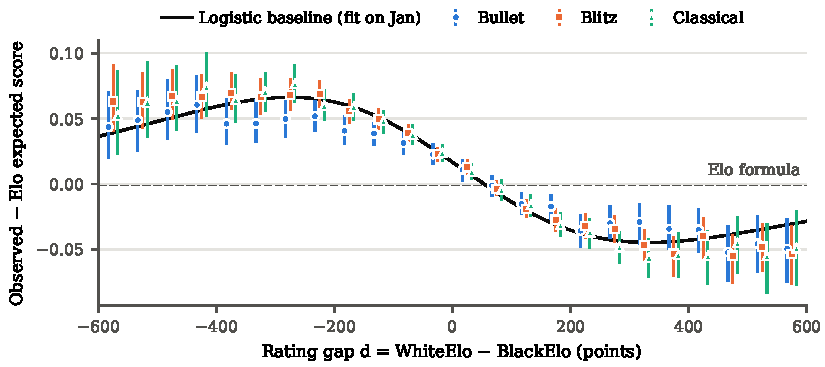
\includegraphics[width=\linewidth]{fig_calibration.pdf}
  \caption{Where the Elo formula misses. Points show the observed February score minus the Elo prediction in 50-point bins of the rating gap, by time class, with 95\% player-level bootstrap intervals; bins with fewer than 200 games are omitted. The dashed line is the Elo formula itself; the solid line is the pooled logistic baseline fitted on January.}
  \label{fig:calibration}
\end{figure}

\paragraph{Flexible models add little.} Against the baseline, the spline gains \dBaseSplineFebAbs{}\tenm{} (interval [\dBaseSplineFebLo{}, \dBaseSplineFebHi{}]) and boosted trees \dBaseBoostFebAbs{}\tenm{} ([\dBaseBoostFebLo{}, \dBaseBoostFebHi{}]). Both intervals exclude zero, and the paired fold differences in January point the same way ((\cvSplineDiff{} $\pm$ \cvSplineSE{}) and (\cvBoostDiff{} $\pm$ \cvBoostSE{})\tenm{}), but they are \gainRatioSpline{} and \gainRatioBoost{} times smaller than the baseline's gain over Elo. The rating logistic gains \dBaseRatingFebAbs{}\tenm{} (interval [\dBaseRatingFebLo{}, \dBaseRatingFebHi{}]), which just reaches zero. The ordinal logit, which models draws explicitly, matches the baseline to four decimals (difference \dBaseOrdinalFeb{}\tenm{}), so treating draws as half-points does not matter. The spline's gain is concentrated in the tails: \gainBigSpline\% of it comes from the \bigGapShare\% of games with $|d| > 400$.

\paragraph{A second test month.} The conditions declared before March was read are all met. The baseline beats Elo by \dEloBaseMarAbs{}\tenm{} with an interval that excludes zero; the ordering of models on log-loss is \orderSame{} as in February; and the slope fitted on March is \SlopeAllMar{} (interval [\SlopeAllMarLo{}, \SlopeAllMarHi{}]), against \SlopeAllJan{} in January.

\begin{table}[t]
  \centering
  \caption{Baseline coefficients by time class, fitted on January; slope ratios are also fitted separately on February and March. White's edge is shown in expected-score points (pp) and in rating points. $\pm$ is half the width of the 95\% player-level interval. }
  \label{tab:advantage}
  \scriptsize
  \resizebox{\textwidth}{!}{\begin{tabular}{lrccccc}
\toprule
 & Games & \multicolumn{2}{c}{White's edge (Jan)} & \multicolumn{3}{c}{Slope / Elo slope} \\
\cmidrule(lr){3-4}\cmidrule(lr){5-7}
Time control & (Jan) & score pts (pp) & rating pts & Jan & Feb & Mar \\
\midrule
Bullet & 405,362 & 1.54 $\pm$ 0.33 & 13.4 $\pm$ 2.9 & 0.802 $\pm$ 0.029 & 0.808 $\pm$ 0.018 & 0.822 $\pm$ 0.019 \\
Blitz & 639,890 & 1.76 $\pm$ 0.24 & 15.8 $\pm$ 2.2 & 0.775 $\pm$ 0.024 & 0.766 $\pm$ 0.018 & 0.769 $\pm$ 0.019 \\
Classical & 433,581 & 1.65 $\pm$ 0.28 & 14.9 $\pm$ 2.5 & 0.769 $\pm$ 0.015 & 0.763 $\pm$ 0.015 & 0.764 $\pm$ 0.015 \\
All games & 1,478,833 & 1.67 $\pm$ 0.16 & 14.8 $\pm$ 1.4 & 0.782 $\pm$ 0.014 & 0.777 $\pm$ 0.011 & 0.782 $\pm$ 0.011 \\
\bottomrule
\end{tabular}
}
\end{table}

\paragraph{White's advantage.} Pooled over time classes, White's expected score at equal ratings is \EdgePPAllJan{} percentage points above $\nicefrac{1}{2}$ (interval [\EdgePPAllJanLo{}, \EdgePPAllJanHi{}]), or \EdgePtsAllJan{} rating points. By time class the edge is \EdgePPBulletJan{}, \EdgePPBlitzJan{} and \EdgePPClassicalJan{} points for bullet, blitz and classical (Table~\ref{tab:advantage}). The intervals overlap heavily. The largest difference, blitz minus bullet, is \conBlitzBullet{} points; its player-level interval is [\conBlitzBulletLo{}, \conBlitzBulletHi{}], and only the day-level interval ([\conBlitzBulletDayLo{}, \conBlitzBulletDayHi{}]) excludes zero, barely. Across five bands of mean rating the edge stays between \bandEdgeMin{} and \bandEdgeMax{} points, and the top band minus the bottom band is \bandEdgeContrast{} ([\bandEdgeLo{}, \bandEdgeHi{}]). Differences between time classes of up to about 0.6 points are therefore not excluded, so ``similar'' is the most we can claim. The slope, by contrast, is highest above 1900 (\SlopeBandE{}) and the top band exceeds the bottom band by \bandContrast{} ([\bandContrastLo{}, \bandContrastHi{}]; Appendix~\ref{app:bands}).

\begin{table}[t]
  \centering
  \caption{Rating-noise checks on January: the slope ratio $\beta_1/(\ln 10/400)$ of the pooled baseline on subsets of games, with 95\% player-level intervals. ``Settled'' is measured by the mean absolute rating change over a player's games on earlier days; thirds are of the larger of the two players' values.}
  \label{tab:noise}
  \small
  \begin{tabular}{lcc}
\toprule
Check (all on January) & Share of games & Slope / Elo slope \\
\midrule
All games & 100\% & 0.782 [0.767, 0.795] \\
Both players $\ge$10 games in January & 96\% & 0.796 [0.780, 0.810] \\
Both players $\ge$100 games & 67\% & 0.817 [0.797, 0.834] \\
\midrule
$\ge$20 earlier-day games each: Displayed gap alone & 67\% & 0.823 [0.808, 0.839] \\
Smoothed (earlier-day) gap alone &  & 0.753 [0.735, 0.773] \\
Both together: sum of the two slopes &  & 0.874 [0.856, 0.891] \\
\midrule
Most settled third (smallest past rating changes) & 22\% & 0.853 [0.823, 0.877] \\
Least settled third & 22\% & 0.793 [0.764, 0.818] \\
\bottomrule
\end{tabular}

\end{table}

\paragraph{Is the shallow slope rating noise?} The checks of Section~4 point the same way (Table~\ref{tab:noise}). (i) Requiring both players to have at least 10, 30 or 100 January games (\shareFreqTen, \shareFreqThirty{} and \shareFreqHundred\% of games) raises the slope only to \slopeFreqTen, \slopeFreqThirty{} and \slopeFreqHundred{}. (ii) On the \histShare\% of games where both players have at least 20 earlier-day games, the smoothed gap alone has a lower slope than the displayed gap (\slopeSmooth{} against \slopeDisp), as a lagging average should; together both carry weight (\slopeBothD{} and \slopeBothS), and the combined slope is \slopeBothSum{} (interval [\slopeBothSumLo{}, \slopeBothSumHi{}]). The past holds information about strength that the displayed rating lacks, as noisy ratings imply, but the slope stays below 1. More settled players have steeper slopes (\slopeTercA{} for the most settled third, \slopeTercC{} for the least; difference \tercContrast{}, interval [\tercContrastLo{}, \tercContrastHi{}]), again as noise predicts, yet even the most settled third is well below 1. (iii) Under classical error, about \sigmaClass{} rating points per player (interval \sigmaClassLo--\sigmaClassHi{}, from the interval of the observed slope) reproduce the slope (Figure~\ref{fig:noise}); with January's exact gap distribution it takes \sigmaPost{}, and under Berkson error \sigmaBerk{}. A comment in current Lichess source says the inactivity decay is chosen so that a typical player's RD goes from 60 to 110 in a year \citep{lila}; Berkson noise of that size flattens the slope only to \simBerkSlopeOneTen{}--\simBerkSlopeSixty{}. So the data are consistent with a correct formula for true strength if displayed ratings carry classical errors of about 56 points, near the low end of that RD range, whereas Berkson noise of typical Glicko size would explain only part of the slope; we cannot tell which structure applies. Classical noise inflates White's edge in rating points far more than in score points (Appendix~\ref{app:sim}), so we lead with score units.

\begin{figure}[t]
  \centering
  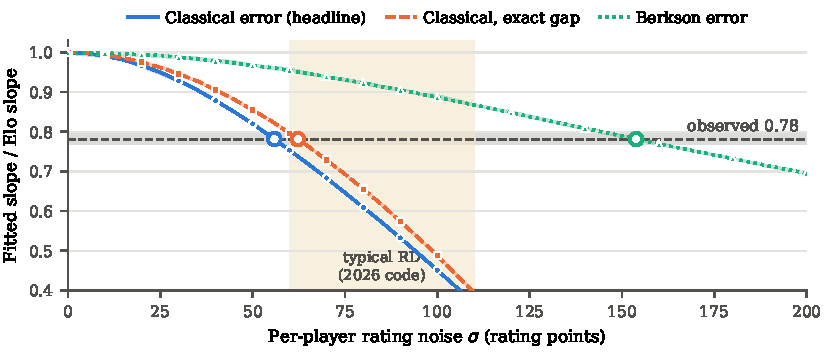
\includegraphics[width=\linewidth]{fig_noise.pdf}
  \caption{Simulation with known truth. Fitted slope divided by the Elo slope when outcomes follow the Elo formula exactly in true strength and displayed ratings carry noise of standard deviation $\sigma$ per player. Lines are means over 20 seeds with min--max bands. Circles mark where each model meets the observed slope (dashed line, with its 95\% player-level interval in grey). The shaded region is the 60--110 range of typical RD named in current Lichess code.}
  \label{fig:noise}
\end{figure}

\paragraph{Error bars and dependence.} Day-level intervals are only \dayOverGameMin--\dayOverGameMax{} times wider than game-level ones, but player-level intervals are \ratioMin--\ratioMax{} times wider than day-level ones (\ratioDelta{} for the baseline's gain over Elo, \ratioSlope{} for the slope, \ratioEdge{} for White's edge; Table~\ref{tab:boot}, Appendix~\ref{app:boot}), so most dependence runs through players, not days. No headline conclusion changes: each difference we call real exceeds its player-level interval, and those we call ties do not.

\section{Limitations}

\textbf{Displayed ratings only.} The public files contain no rating deviations, so we cannot compute Glicko-2's own expected score, which shrinks the gap by a factor that depends on both deviations; our claim is about the Elo formula applied to displayed ratings. \textbf{The noise story is bounded, not identified.} The simulation assumes Gaussian noise of equal size for every player and a fixed White edge; the two classical constructions differ (\sigmaClass{} against \sigmaPost{} points), and classical and Berkson error differ by almost a factor of three. The 60--110 RD range comes from 2026 source code, not 2015 settings. \textbf{Provisional players.} Dropping games with a rating of exactly 1500, the default for new accounts, raises the slope to \SlopeNoFifteen{}; the history proxy for how settled a player is also depends on opponents. \textbf{Dependence and scope.} The pigeonhole bootstrap is conservative but ignores clustering by tournament and time of day; a month has only 28--31 days. We use three months of 2015 and make no claim about today's Lichess. \textbf{Process.} February was scored in our early draft, so only March is untouched; the robustness checks and the three noise constructions were chosen after seeing January and February, and the time-class rule after a first March run. \textbf{Causes.} We show that Elo is overconfident on displayed ratings and that noise could explain it; we do not show that it does.

\section{Conclusion}

Applied to displayed Lichess ratings, the Elo formula is overconfident: the fitted slope is \SlopeAllJan{} of Elo's (interval [\SlopeAllJanLo{}, \SlopeAllJanHi{}]), and \SlopeAllFeb{} and \SlopeAllMar{} in the two test months. A two-parameter logistic fit beats the formula by \dEloBaseFebAbs{}\tenm{} of log-loss in February and \dEloBaseMarAbs{}\tenm{} in March; splines, boosted trees and an ordinal model add at most \gainPctBoost\% more. Whether the formula is wrong about true strength is open: classical rating errors of about \sigmaClass{} points would produce the slope with no miscalibration, Berkson errors of Glicko size would explain only part of it, and the deviations needed to decide are not in the public files. White's edge is \EdgePPAllJan{} points of expected score across time controls.

\section*{Acknowledgements and statements}

\textbf{AI use.} We used Claude (Anthropic) for guidance: it drafted and debugged code, ran analyses, suggested and checked references, and edited the manuscript, including the additions in this version (player-level bootstrap, March test month, extended simulations). Project direction, design, verification and decisions were made by the team.

\textbf{Contributions.} Xinran Gao: data pipeline review, exploratory analysis and final figures. Pedro S{\'a}nchez-Gil Galindo: Elo baseline, calibration curves and sensitivity analyses. Liam Campbell: extended models, cross-validation, bootstrap and noise analyses. All authors wrote and checked the paper. \todo{Authors: say who reviewed the additions in this version (player-level bootstrap, March, simulation variants, limitations).}

\textbf{Data and code.} Data are the Lichess open database (CC0 1.0), headers only. Code and every result file are in the repository on the first page; the final-version pipeline, the March declaration and the frozen selection are in its \texttt{final/} directory, and \texttt{final/run\_all.sh} rebuilds this paper from the raw files.

\begin{thebibliography}{99}

\bibitem[Bates et~al.(2024)]{bates2024}
S.~Bates, T.~Hastie, and R.~Tibshirani.
\newblock Cross-validation: What does it estimate and how well does it do it?
\newblock \emph{Journal of the American Statistical Association}, 119(546):1434--1445, 2024.

\bibitem[Berkson(1950)]{berkson1950}
J.~Berkson.
\newblock Are there two regressions?
\newblock \emph{Journal of the American Statistical Association}, 45(250):164--180, 1950.

\bibitem[Bradley and Terry(1952)]{bradley1952}
R.~A. Bradley and M.~E. Terry.
\newblock Rank analysis of incomplete block designs: I. The method of paired comparisons.
\newblock \emph{Biometrika}, 39(3/4):324--345, 1952.

\bibitem[Cameron et~al.(2011)]{cameron2011}
A.~C. Cameron, J.~B. Gelbach, and D.~L. Miller.
\newblock Robust inference with multiway clustering.
\newblock \emph{Journal of Business \& Economic Statistics}, 29(2):238--249, 2011.

\bibitem[Carroll et~al.(2006)]{carroll2006}
R.~J. Carroll, D.~Ruppert, L.~A. Stefanski, and C.~M. Crainiceanu.
\newblock \emph{Measurement Error in Nonlinear Models: A Modern Perspective}.
\newblock Chapman \& Hall/CRC, 2nd edition, 2006. doi: 10.1201/9781420010138.

\bibitem[Efron and Tibshirani(1993)]{efron1993}
B.~Efron and R.~J. Tibshirani.
\newblock \emph{An Introduction to the Bootstrap}.
\newblock Chapman \& Hall, 1993.

\bibitem[Elo(1978)]{elo1978}
A.~E. Elo.
\newblock \emph{The Rating of Chessplayers, Past and Present}.
\newblock Arco, New York, 1978.

\bibitem[Friedman(2001)]{friedman2001}
J.~H. Friedman.
\newblock Greedy function approximation: A gradient boosting machine.
\newblock \emph{The Annals of Statistics}, 29(5):1189--1232, 2001.

\bibitem[Glickman(1999)]{glickman1999}
M.~E. Glickman.
\newblock Parameter estimation in large dynamic paired comparison experiments.
\newblock \emph{Journal of the Royal Statistical Society: Series C (Applied Statistics)}, 48(3):377--394, 1999.

\bibitem[Glickman(2001)]{glickman2001}
M.~E. Glickman.
\newblock Dynamic paired comparison models with stochastic variances.
\newblock \emph{Journal of Applied Statistics}, 28(6):673--689, 2001.

\bibitem[Gneiting and Raftery(2007)]{gneiting2007}
T.~Gneiting and A.~E. Raftery.
\newblock Strictly proper scoring rules, prediction, and estimation.
\newblock \emph{Journal of the American Statistical Association}, 102(477):359--378, 2007.

\bibitem[Guo et~al.(2017)]{guo2017}
C.~Guo, G.~Pleiss, Y.~Sun, and K.~Q. Weinberger.
\newblock On calibration of modern neural networks.
\newblock In \emph{Proceedings of the 34th International Conference on Machine Learning}, volume~70 of \emph{PMLR}, 2017. arXiv:1706.04599.

\bibitem[Hastie et~al.(2009)]{hastie2009}
T.~Hastie, R.~Tibshirani, and J.~Friedman.
\newblock \emph{The Elements of Statistical Learning}.
\newblock Springer, 2nd edition, 2009.

\bibitem[Hvattum and Arntzen(2010)]{hvattum2010}
L.~M. Hvattum and H.~Arntzen.
\newblock Using {ELO} ratings for match result prediction in association football.
\newblock \emph{International Journal of Forecasting}, 26(3):460--470, 2010.

\bibitem[James et~al.(2021)]{islr}
G.~James, D.~Witten, T.~Hastie, and R.~Tibshirani.
\newblock \emph{An Introduction to Statistical Learning}.
\newblock Springer, 2nd edition, 2021.

\bibitem[Ke et~al.(2017)]{ke2017}
G.~Ke, Q.~Meng, T.~Finley, T.~Wang, W.~Chen, W.~Ma, Q.~Ye, and T.-Y. Liu.
\newblock {LightGBM}: A highly efficient gradient boosting decision tree.
\newblock In \emph{Advances in Neural Information Processing Systems}, volume~30, 2017.

\bibitem[Lichess(2015)]{lichessdb}
Lichess.
\newblock Lichess open database: Standard rated games, January--March 2015.
\newblock \url{https://database.lichess.org/}, released under CC0 1.0. Accessed 26 November 2026.

\bibitem[Lichess(2026)]{lila}
Lichess.
\newblock lila source code, \texttt{modules/rating/src/main/Glicko.scala}.
\newblock \url{https://github.com/lichess-org/lila}. Accessed 26 November 2026.

\bibitem[Owen(2007)]{owen2007}
A.~B. Owen.
\newblock The pigeonhole bootstrap.
\newblock \emph{The Annals of Applied Statistics}, 1(2):386--411, 2007.

\bibitem[Papke and Wooldridge(1996)]{papke1996}
L.~E. Papke and J.~M. Wooldridge.
\newblock Econometric methods for fractional response variables with an application to 401(k) plan participation rates.
\newblock \emph{Journal of Applied Econometrics}, 11(6):619--632, 1996.

\bibitem[Pedregosa et~al.(2011)]{pedregosa2011}
F.~Pedregosa, G.~Varoquaux, A.~Gramfort, V.~Michel, B.~Thirion, O.~Grisel, M.~Blondel, P.~Prettenhofer, R.~Weiss, V.~Dubourg, J.~Vanderplas, A.~Passos, D.~Cournapeau, M.~Brucher, M.~Perrot, and \'E.~Duchesnay.
\newblock Scikit-learn: Machine learning in {Python}.
\newblock \emph{Journal of Machine Learning Research}, 12:2825--2830, 2011.

\bibitem[Sonas(2011)]{sonas2011}
J.~Sonas.
\newblock The Elo rating system -- correcting the expectancy tables.
\newblock \emph{ChessBase News}, March 2011.
\newblock \url{https://en.chessbase.com/post/the-elo-rating-system-correcting-the-expectancy-tables}.

\end{thebibliography}

\appendix

\section{Data cleaning and the March relabelling}
\label{app:data}

\begin{table}[h]
  \centering
  \caption{Games removed at each cleaning step, in order.}
  \small
  \begin{tabular}{lrrr}
\toprule
 & Jan 2015 & Feb 2015 & Mar 2015 \\
\midrule
Games in the file & 1,497,237 & 1,495,553 & 1,742,733 \\
Correspondence (not bullet, blitz or classical) & 5,458 & 6,498 & 7,589 \\
Abandoned & 11,708 & 10,187 & 10,828 \\
Missing rating & 0 & 1 & 1 \\
Dated outside the month & 1,238 & 1,998 & 2,146 \\
\midrule
Games kept & 1,478,833 & 1,476,869 & 1,722,169 \\
Bullet games kept & 405,362 & 391,126 & 444,254 \\
Blitz games kept & 639,890 & 649,835 & 771,423 \\
Classical games kept & 433,581 & 435,908 & 506,492 \\
\bottomrule
\end{tabular}

\end{table}

Time classes follow estimated duration; the label-based and duration-based classes agree on every kept game in all three months. Counting only March games labelled bullet, blitz or ``Classical'' (dropping the \nStandardMar{} ``Standard'' games; \nMarLabels{} games remain), the baseline's gain over Elo is \dEloBaseMarLabels\tenm{} (interval [\dEloBaseMarLabelsLo{}, \dEloBaseMarLabelsHi{}]), against \dEloBaseMar\tenm{} for all games.

\section{Further model metrics}
\label{app:models}

\begin{table}[h]
  \centering
  \caption{Paired CV differences against the baseline (mean $\pm$ standard error over 5 folds, units of $10^{-4}$), and Brier score and calibration error on both test months; $\pm$ as in Table~\ref{tab:models}.}
  \scriptsize
  \resizebox{\textwidth}{!}{\begin{tabular}{llcccccc}
\toprule
 & & CV paired diff. & \multicolumn{2}{c}{Feb} & \multicolumn{3}{c}{Mar} \\
\cmidrule(lr){4-5}\cmidrule(lr){6-8}
Model & Params & vs.\ baseline ($10^{-4}$) & Brier & Calib. & log-loss & Brier & Calib. \\
\midrule
Floor (White's mean score) & 1 & 729.68 $\pm$ 4.16 & 0.2403 $\pm$ 0.0003 & -- & 0.6925 $\pm$ 0.0001 & 0.2404 $\pm$ 0.0002 & -- \\
Elo formula & 0 & 43.48 $\pm$ 0.53 & 0.2089 $\pm$ 0.0013 & 0.0304 & 0.6257 $\pm$ 0.0032 & 0.2086 $\pm$ 0.0013 & 0.0297 \\
Logistic on $d$, pooled & 2 & 0.10 $\pm$ 0.13 & 0.2076 $\pm$ 0.0013 & 0.0033 & 0.6213 $\pm$ 0.0030 & 0.2073 $\pm$ 0.0013 & 0.0034 \\
Logistic on $d$ by time control & 6 & -- & 0.2076 $\pm$ 0.0013 & 0.0034 & 0.6213 $\pm$ 0.0030 & 0.2073 $\pm$ 0.0013 & 0.0036 \\
Rating logistic (adds mean rating) & 9 & $-$0.25 $\pm$ 0.08 & 0.2076 $\pm$ 0.0013 & 0.0033 & 0.6213 $\pm$ 0.0030 & 0.2073 $\pm$ 0.0013 & 0.0036 \\
Spline logistic & 17 & $-$1.97 $\pm$ 0.19 & 0.2076 $\pm$ 0.0013 & 0.0017 & 0.6211 $\pm$ 0.0030 & 0.2073 $\pm$ 0.0013 & 0.0007 \\
Boosted trees & -- & $-$3.19 $\pm$ 0.32 & 0.2075 $\pm$ 0.0013 & 0.0017 & 0.6210 $\pm$ 0.0030 & 0.2072 $\pm$ 0.0013 & 0.0010 \\
Ordinal logit (draws modelled) & 9 & 0.01 $\pm$ 0.00 & 0.2076 $\pm$ 0.0013 & 0.0033 & 0.6213 $\pm$ 0.0030 & 0.2073 $\pm$ 0.0013 & 0.0035 \\
\bottomrule
\end{tabular}
}
\end{table}

\section{Rating bands and robustness (January)}
\label{app:bands}

\begin{table}[h]
  \centering
  \caption{Course baseline refitted on subsets of January; $\pm$ is half the width of the 95\% player-level interval. Bands are of the pair's mean rating.}
  \small
  \resizebox{\textwidth}{!}{\begin{tabular}{lrccc}
\toprule
Subset of January & Games & White's edge (pp) & White's edge (rating pts) & Slope / Elo slope \\
\midrule
$<$1300 & 102,534 & 1.82 $\pm$ 0.55 & 16.0 $\pm$ 4.9 & 0.786 $\pm$ 0.032 \\
1300--1500 & 332,439 & 1.69 $\pm$ 0.32 & 15.6 $\pm$ 3.1 & 0.754 $\pm$ 0.019 \\
1500--1700 & 515,257 & 1.59 $\pm$ 0.27 & 14.2 $\pm$ 2.5 & 0.774 $\pm$ 0.023 \\
1700--1900 & 366,605 & 1.65 $\pm$ 0.33 & 14.5 $\pm$ 3.0 & 0.793 $\pm$ 0.022 \\
$\ge$1900 & 161,998 & 1.87 $\pm$ 0.47 & 15.5 $\pm$ 3.9 & 0.840 $\pm$ 0.026 \\
\midrule
All games (reference) & 1,478,833 & 1.67 $\pm$ 0.16 & 14.8 $\pm$ 1.4 & 0.782 $\pm$ 0.014 \\
Drop rules-infraction games & 1,478,732 & 1.66 $\pm$ 0.16 & 14.8 $\pm$ 1.4 & 0.782 $\pm$ 0.014 \\
Drop games with a rating of exactly 1500 & 1,441,884 & 1.65 $\pm$ 0.16 & 14.3 $\pm$ 1.5 & 0.801 $\pm$ 0.015 \\
Drop time-forfeit games & 995,760 & 2.02 $\pm$ 0.21 & 18.0 $\pm$ 2.0 & 0.781 $\pm$ 0.020 \\
January 1--15 only & 696,133 & 1.63 $\pm$ 0.23 & 14.5 $\pm$ 2.1 & 0.783 $\pm$ 0.018 \\
January 16--31 only & 782,700 & 1.70 $\pm$ 0.21 & 15.1 $\pm$ 1.9 & 0.780 $\pm$ 0.016 \\
\bottomrule
\end{tabular}
}
\end{table}

Dropping the \nInfrJan{} rules-infraction games changes nothing. Dropping games with a rating of exactly 1500, the default for new accounts, raises the slope to \SlopeNoFifteen{}. Dropping time-forfeit games leaves the slope at \SlopeNoForfeit{} but raises White's edge to \EdgePtsNoForfeit{} rating points (\EdgePPNoForfeit{} percentage points), so White's edge is larger in games decided on the board. The two halves of January agree (\SlopeHalfA{} and \SlopeHalfB{}).

\section{Simulation details}
\label{app:sim}

For each simulated game, $S \sim \text{Bernoulli}(E[S \mid T + a])$ with $E$ the Elo formula, $T$ the true gap and $a$ White's true edge (\simTrueEdgePts{} rating points, the observed pooled edge converted to rating points). Write $\mu$ and $v$ for the mean and variance of January's observed gaps and $\lambda = 1 - 2\sigma^2/v$. \emph{Classical error (headline):} $T = \mu + \sqrt{\lambda}(d - \mu)$ with $d$ drawn from January's observed gaps, and the displayed gap is $T + N(0, 2\sigma^2)$; its variance is $v$ for every $\sigma$ (checked in the simulation), its mean is $\mu$, and its shape is a smoothed version of January's. \emph{Classical, exact gap:} the displayed gap is the observed $d$, and $T \mid d \sim N(\mu + \lambda(d - \mu),\, 2\lambda\sigma^2)$, the exact posterior if $T$ is Gaussian; the displayed gap then has January's exact distribution. \emph{Berkson error:} the displayed gap is the observed $d$ and $T = d + N(0, 2\sigma^2)$. Each fit is the pooled baseline~\eqref{eq:logit} on simulated January data (\nGamesJan{} games). Under classical error at $\sigma = 50$ the fitted edge is \simClassEdgePtsFifty{} rating points against a true \simTrueEdgePts{}, but \simClassEdgePPFifty{} points of score against \simTruePP{} (\simClassEdgePPErr\% off); under Berkson error the rating-point edge is unchanged and the score edge falls (Table~\ref{tab:sim}). The $\sigma$ at which the mean fitted slope ratio crosses the observed value is found by linear interpolation; the interval is the crossing for the ends of the observed slope's 95\% player-level interval.

\begin{table}[h]
  \centering
  \caption{Simulated fitted slope ratio and fitted White's edge (percentage points of expected score; rating points) against per-player noise $\sigma$, means over 20 seeds. The true edge is \simTruePP{} points of score, \simTrueEdgePts{} rating points; ``--'' where the construction needs more noise than the gap variance allows.}
  \label{tab:sim}
  \scriptsize
  \resizebox{\textwidth}{!}{\begin{tabular}{lccccccccc}
\toprule
 & \multicolumn{3}{c}{Classical (headline)} & \multicolumn{3}{c}{Classical, exact gap} & \multicolumn{3}{c}{Berkson} \\
\cmidrule(lr){2-4}\cmidrule(lr){5-7}\cmidrule(lr){8-10}
$\sigma$ & slope & edge pp & edge pts & slope & edge pp & edge pts & slope & edge pp & edge pts \\
\midrule
0 & 1.000 & 1.67 & 11.6 & 1.000 & 1.65 & 11.5 & 1.000 & 1.65 & 11.5 \\
30 & 0.929 & 1.69 & 12.7 & 0.946 & 1.67 & 12.3 & 0.987 & 1.64 & 11.6 \\
50 & 0.820 & 1.71 & 14.5 & 0.855 & 1.69 & 13.8 & 0.967 & 1.61 & 11.6 \\
55 & 0.788 & 1.74 & 15.3 & 0.828 & 1.71 & 14.4 & 0.962 & 1.59 & 11.5 \\
60 & 0.754 & 1.74 & 16.1 & 0.796 & 1.71 & 14.9 & 0.955 & 1.58 & 11.5 \\
70 & 0.684 & 1.78 & 18.1 & 0.729 & 1.74 & 16.6 & 0.939 & 1.56 & 11.6 \\
110 & 0.368 & 1.95 & 36.8 & 0.395 & 1.93 & 33.9 & 0.868 & 1.44 & 11.6 \\
150 & -- & -- & -- & -- & -- & -- & 0.790 & 1.32 & 11.6 \\
\bottomrule
\end{tabular}
}
\end{table}

\section{Bootstrap schemes}
\label{app:boot}

Table~\ref{tab:boot} gives the half-width of the 95\% interval for the headline quantities under the game, day and player schemes (2000 resamples for test-set quantities, 1000 for coefficients).

\begin{table}[h]
  \centering
  \caption{Half-widths of 95\% bootstrap intervals under three resampling schemes, on the same data. Player resampling widens intervals by a factor of \ratioMin--\ratioMax{} relative to day resampling.}
  \label{tab:boot}
  \small
  \begin{tabular}{lcccc}
\toprule
Quantity (half-width of 95\% interval) & Game & Day & Player & Player / day \\
\midrule
Baseline $-$ Elo, Feb log-loss ($10^{-4}$) & 1.5 & 1.9 & 4.3 & 2.2 \\
Baseline $-$ Elo, Mar log-loss ($10^{-4}$) & 1.5 & 1.5 & 4.6 & 3.0 \\
Boosted $-$ baseline, Feb ($10^{-4}$) & 0.45 & 0.46 & 1.06 & 2.3 \\
Slope / Elo slope, Jan ($10^{-3}$) & 3.8 & 4.1 & 14.3 & 3.5 \\
White's edge, Jan (pp) & 0.08 & 0.09 & 0.16 & 1.7 \\
\bottomrule
\end{tabular}

\end{table}

\end{document}
